\documentclass[11pt,a4paper]{article}

% =========================================================================
% PACKAGE CONFIGURATION & TYPOGRAPHY
% =========================================================================
\usepackage[utf8]{inputenc}
\usepackage[margin=1in,headheight=14.5pt]{geometry}
\usepackage{graphicx}
\usepackage{booktabs}
\usepackage{tabularx}
\usepackage{array}
\usepackage{colortbl}
\usepackage{amsmath}
\usepackage{amssymb}
\usepackage{float}
\usepackage{xcolor}
\usepackage{fancyhdr}
\usepackage{listings}
\usepackage{enumitem}
\usepackage{microtype}
\usepackage{ragged2e}
\usepackage{subcaption}
\usepackage{tikz}
\usetikzlibrary{shapes.geometric, arrows, positioning, fit, calc}
\usepackage{xurl}
\usepackage[colorlinks=true,linkcolor=vesitnavy,citecolor=vesitnavy,urlcolor=vesitnavy,plainpages=false,pdfpagelabels=true,pdftitle={KGIRS Micro Project Report - Automatic Evaluation of RAG Answers},pdfauthor={Tanishque Suthar, Vanshika Somnani, Harsh Tanwani}]{hyperref}

\setcounter{tocdepth}{2}

% Institutional Colors (VESIT Palette)
\definecolor{vesitnavy}{RGB}{12, 44, 98}
\definecolor{vesitgold}{RGB}{197, 145, 22}
\definecolor{tableheader}{RGB}{236, 242, 250}
\definecolor{codebg}{RGB}{248, 250, 252}
\definecolor{codeframe}{RGB}{218, 224, 233}
\definecolor{codecomment}{RGB}{75, 115, 115}
\definecolor{codekw}{RGB}{16, 42, 142}

% Code Listing Configuration
\lstset{
    backgroundcolor=\color{codebg},
    basicstyle=\ttfamily\footnotesize,
    breaklines=true,
    breakatwhitespace=true,
    frame=single,
    rulecolor=\color{codeframe},
    numbers=left,
    numberstyle=\tiny\color{gray!70},
    numbersep=7pt,
    tabsize=2,
    showstringspaces=false,
    keywordstyle=\color{codekw}\bfseries,
    commentstyle=\color{codecomment}\itshape,
    stringstyle=\color{vesitgold!90!black},
    xleftmargin=12pt,
    framexleftmargin=12pt
}

% Page Layout & Running Headers
\pagestyle{fancy}
\fancyhf{}
\fancyhead[L]{\footnotesize\color{gray}VESIT -- Department of Computer Engineering}
\fancyhead[R]{\footnotesize\color{gray}KGIRS Micro Project Report}
\fancyfoot[L]{\footnotesize\color{gray}Academic Year 2026--2027}
\fancyfoot[R]{\footnotesize\thepage}
\renewcommand{\headrulewidth}{0.4pt}
\renewcommand{\footrulewidth}{0.4pt}

\setlength{\parindent}{0pt}
\setlength{\parskip}{5pt}
\renewcommand{\arraystretch}{1.2}

\begin{document}
\hypersetup{pageanchor=false}

% =========================================================================
% COVER PAGE
% =========================================================================
\begin{titlepage}
\begin{center}
    {\large \textbf{VIVEKANAND EDUCATION SOCIETY'S INSTITUTE OF TECHNOLOGY}}\\[0.15cm]
    {\normalsize \textbf{An Autonomous Institute Affiliated to the University of Mumbai}}\\[0.1cm]
    {\footnotesize \textbf{Hashu Advani Memorial Complex, Collector's Colony, Chembur, Mumbai - 400 074}}\\[0.35cm]
    
    \includegraphics[width=2.3cm]{report_images/vesit_logo.png}\\[0.35cm]
    
    {\large \textbf{DEPARTMENT OF COMPUTER ENGINEERING}}\\[0.25cm]
    {\Large \textbf{\color{vesitnavy}MICRO PROJECT REPORT}}\\[0.35cm]
    
    \noindent\rule{\linewidth}{1.2pt}\\[0.25cm]
    {\Large \textbf{How Much Can We Trust Automatic Evaluation of RAG Answers?}}\\[0.2cm]
    {\large \textit{An Empirical Benchmark of RAGAS, LLM-as-a-Judge, and Retrieval Alignment on RAGTruth}}\\[0.2cm]
    \noindent\rule{\linewidth}{1.2pt}\\[0.35cm]

    \textbf{SDG Alignment:} SDG 9 (Industry, Innovation, and Infrastructure) \& SDG 4 (Quality Education)\\[0.45cm]

    % Project Course Details Table
    \begin{tabularx}{\linewidth}{|>{\bfseries}p{5.0cm}|X|}
    \hline
    \rowcolor{vesitnavy!12}
    \multicolumn{2}{|c|}{\textbf{\color{vesitnavy}Project / Course Details}} \\
    \hline
    Course / Subject Name & Knowledge Graph and Information Retrieval Systems (KGIRS) \\
    \hline
    Course Code / Semester / AY & CSC701 / Semester VII / Academic Year 2026--2027 \\
    \hline
    Faculty Incharge / Project Mentor & \\
    \hline
    Project Group No. & \\
    \hline
    Submission Date & \\
    \hline
    Source Code Repository & \url{https://github.com/tanishque-suthar/kgirs-minip} \\
    \hline
    \end{tabularx}\\[0.45cm]

    % Team Details Table
    \begin{tabularx}{\linewidth}{|>{\RaggedRight}p{4.2cm}|>{\centering\arraybackslash}p{2.0cm}|>{\centering\arraybackslash}p{2.5cm}|>{\RaggedRight}X|}
    \hline
    \rowcolor{vesitnavy!12}
    \multicolumn{4}{|c|}{\textbf{\color{vesitnavy}Project Team Details}} \\
    \hline
    \textbf{Student Name} & \textbf{Roll No.} & \textbf{Class / Div} & \textbf{Institute Email ID} \\
    \hline
    Tanishque Suthar & 53 & D17B & \href{mailto:2023.tanishque.suthar@ves.ac.in}{2023.tanishque.suthar@ves.ac.in} \\
    \hline
    Vanshika Somnani & 52 & D17B & \href{mailto:2023.vanshika.somnani@ves.ac.in}{2023.vanshika.somnani@ves.ac.in} \\
    \hline
    Harsh Tanwani & 54 & D17B & \href{mailto:2023.harsh.tanwani@ves.ac.in}{2023.harsh.tanwani@ves.ac.in} \\
    \hline
    \end{tabularx}

    \vfill
    {\footnotesize Department of Computer Engineering, VESIT $\vert$ Academic Year: 2026--2027}
\end{center}
\end{titlepage}
\hypersetup{pageanchor=true}

% =========================================================================
% FRONT MATTER (ROMAN NUMBERING)
% =========================================================================
\pagenumbering{roman}

% Abstract
\section*{Abstract}
\addcontentsline{toc}{section}{Abstract}
Retrieval-Augmented Generation (RAG) frameworks have emerged as the state-of-the-art paradigm for factual question answering in high-stakes enterprise applications. Consequently, practitioners increasingly rely on automated evaluators---primarily continuous scoring frameworks like RAGAS (Faithfulness and Answer Relevancy) and discrete LLM-as-a-Judge prompting---to benchmark pipelines without continuous, labor-intensive human intervention. However, critical questions persist regarding the actual reliability, systematic prompt biases, and statistical alignment of these evaluators. 

This micro-project presents an empirical investigation into automatic RAG evaluation using a stratified benchmark of 100 question-answering samples from the official RAGTruth corpus, partitioned across three balanced hallucination severity tiers (40 correct, 30 partly faithful, 30 incorrect). We evaluate RAGAS continuous metrics, measure rank correlation (Spearman $r_s$ and Kendall $\tau_b$) via 1,000-resample non-parametric bootstrapping, quantify position and verbosity biases in Gemini-based LLM judges, compute inter-annotator agreement (pairwise quadratic Cohen's $\kappa$ and Fleiss' $\kappa$) across human ground truth, an independent blind human relabeller ($n=35$), and the LLM judge, and assess the correlation between retrieval metrics (MRR, NDCG) and final answer correctness. 

The findings reveal that automated metrics exhibit significant blind spots: RAGAS Faithfulness struggles to penalize nuanced single-span hallucinations ($r_s = 0.00$), prompt judges are prone to central-tendency mode collapse, and retrieval rank exhibits near-zero coupling with generational hallucinations ($r_s = -0.02$). Human-to-human agreement remains substantial ($\kappa = 0.7368$), whereas LLM-to-human agreement drops to chance levels ($\kappa = 0.00$). The project delivers an interactive multi-page Streamlit analytical workbench equipped with disk-level caching to promote sustainable, zero-redundancy LLM benchmarking aligned with UN SDG 9 (Industry, Innovation, and Infrastructure) and SDG 12 (Responsible Consumption).

\vspace{0.4cm}
\textbf{Keywords:} Retrieval-Augmented Generation (RAG), Automated Evaluation, RAGAS, LLM-as-a-Judge, Hallucination Detection, Inter-Annotator Agreement, Information Retrieval.
\newpage

% Table of Contents
\begingroup
\setlength{\parskip}{0pt}
\renewcommand{\baselinestretch}{0.94}\normalsize
\makeatletter
\renewcommand*\l@section[2]{%
  \ifnum \c@tocdepth >\z@
    \addpenalty\@secpenalty
    \addvspace{0.45em \@plus\p@}%
    \setlength\@tempdima{1.5em}%
    \begingroup
      \parindent \z@ \rightskip \@pnumwidth
      \parfillskip -\@pnumwidth
      \leavevmode \bfseries
      \advance\leftskip\@tempdima
      \hskip -\leftskip
      #1\nobreak\hfil \nobreak\hb@xt@\@pnumwidth{\hss #2}\par
    \endgroup
  \fi}
\makeatother
\tableofcontents
\endgroup
\newpage

% =========================================================================
% MAIN BODY (ARABIC NUMBERING)
% =========================================================================
\pagenumbering{arabic}

% =========================================================================
% SECTION 1: INTRODUCTION
% =========================================================================
\section{Introduction}

\subsection{Background and Motivation}
In recent years, Retrieval-Augmented Generation (RAG) \cite{lewis2020retrieval} has become the architectural cornerstone of knowledge-intensive Natural Language Processing (NLP) and modern Information Retrieval (IR) systems. By bridging parametric knowledge stored within large language models (LLMs) with non-parametric knowledge retrieved dynamically from external vector stores, inverted indexes, or knowledge graphs, RAG systems substantially reduce factual hallucinations and keep outputs grounded in proprietary corpora. 

Despite their theoretical strengths, evaluating RAG applications in production presents severe engineering challenges. Traditional lexical metrics (e.g., BLEU, ROUGE) rely on exact n-gram matching against golden references, which fails to capture semantic correctness and factual faithfulness. Conversely, manual human evaluation provides golden ground truth but is prohibitively expensive, time-consuming, and difficult to scale. To circumvent these bottlenecks, two automated paradigms have gained widespread industry adoption:
\begin{enumerate}[leftmargin=*]
    \item \textbf{Continuous Heuristic Metric Engines (e.g., RAGAS)}: Metrics such as \textit{Faithfulness} (decomposing answers into atomic factual claims and verifying each against context) and \textit{Answer Relevancy} (generating candidate questions from the answer and computing cosine similarity against the original query).
    \item \textbf{LLM-as-a-Judge Prompting}: Zero-shot or few-shot direct evaluation where a frontier LLM (e.g., Gemini, GPT-4) assigns discrete ordinal quality grades (such as \texttt{correct}, \texttt{partly}, \texttt{incorrect}) accompanied by explanatory natural language rationales.
\end{enumerate}

While automated evaluators are now routinely used to optimize retrieval top-$k$, select embedding models, and steer prompt engineering, practitioners rarely audit the evaluators themselves. When an automated metric assigns a score of 0.85, does it truly mean the response is factually trustworthy? This project investigates this fundamental question.

\subsection{Problem Context}
In production RAG systems, subtle hallucinations can be catastrophic. Consider an enterprise medical or financial assistant: an answer that is 90\% linguistically fluent but contains a single fabricated numerical dosage or contradictory policy detail can lead to severe liability. Automated evaluators frequently conflate \textit{fluency} with \textit{faithfulness}. Furthermore, recent literature indicates that LLM judges suffer from systematic cognitive biases, including:
\begin{itemize}[leftmargin=*]
    \item \textbf{Position Bias}: Sensitivity to the order in which rubrics or multiple candidate options are presented in the evaluation prompt.
    \item \textbf{Verbosity Bias}: An inclination to assign higher accuracy scores to longer, fluff-filled, or syntactically elaborate answers regardless of their factual ground truth.
    \item \textbf{Retrieval-Generation Decoupling}: The prevailing assumption that superior passage retrieval (high MRR and NDCG) guarantees faithful answer generation.
\end{itemize}

A critical empirical gap exists: practitioners need a transparent, reproducible benchmark to measure how closely continuous and discrete automated evaluators agree with verified human ground truth across varying hallucination severities.

\subsection{Intended Users / Stakeholders}
The primary stakeholders and beneficiaries of this work include:
\begin{itemize}[leftmargin=*]
    \item \textbf{RAG System Architects and AI Engineers}: Who require validated evaluation guardrails before deploying generative pipelines to production.
    \item \textbf{Information Retrieval (IR) Researchers}: Investigating the mathematical correlation between retrieval ranking quality (MRR, NDCG) and downstream generative factuality.
    \item \textbf{Quality Assurance and Compliance Auditors}: Tasked with certifying enterprise AI systems against factual drift, regulatory standards, and bias.
    \item \textbf{Academic Students and Educators}: Seeking a pedagogical benchmark and interactive laboratory platform for Information Retrieval and Knowledge Graph courses.
\end{itemize}

% =========================================================================
% SECTION 2: PROBLEM DEFINITION, OBJECTIVES AND SCOPE
% =========================================================================
\section{Problem Definition, Objectives and Scope}

\subsection{Problem Statement}
Given a collection of question-answering interactions comprising retrieved context passages, user questions, generative model answers, and human-annotated word-level hallucination spans from the RAGTruth benchmark, the objective of this project is to quantitatively measure the reliability, rank correlation, prompt-order sensitivity, verbosity vulnerability, and inter-rater consensus of automatic evaluation metrics (RAGAS and Gemini LLM Judge) against stratified human ground truth.

\subsection{Objectives}
The specific, measurable technical objectives of this project are:
\begin{enumerate}[leftmargin=*]
    \item \textbf{Benchmark Formulation}: Construct a stratified 100-sample evaluation dataset from the official RAGTruth QA subset, partitioned deterministically (seed = 42) into 40 \texttt{correct}, 30 \texttt{partly}, and 30 \texttt{incorrect} answers.
    \item \textbf{Correlation Analysis}: Compute Spearman rank correlation ($r_s$) and Kendall tau-b ($\tau_b$) between continuous RAGAS metrics (Faithfulness, Answer Relevancy) and ordinal human ground truth labels, generating 95\% confidence intervals via 1,000-resample non-parametric bootstrapping.
    \item \textbf{LLM Judge Classification Audit}: Evaluate the classification accuracy, 3$\times$3 confusion matrix, and Quadratic-Weighted Cohen's Kappa ($\kappa$) of a Gemini-based LLM judge.
    \item \textbf{Prompt Bias Quantification}: Empirically quantify \textit{position bias} by measuring the rubric flip rate when option definitions are reversed, and \textit{verbosity bias} by analyzing answer length correlations and conducting a neutral fluff-padding perturbation test ($n=19$).
    \item \textbf{Multi-Rater Agreement (Mini-IAA)}: Compute pairwise Quadratic Cohen's Kappa and overall Fleiss' Kappa across three independent raters: Rater A (RAGTruth ground truth), Rater B (blind manual human relabeller, $n=35$), and Rater C (Gemini LLM Judge).
    \item \textbf{Retrieval-to-Generation Decoupling}: Measure Mean Reciprocal Rank (MRR) and Normalized Discounted Cumulative Gain (NDCG) using proxy passage relevance, and analyze their correlation with answer faithfulness.
    \item \textbf{Interactive Dashboard Implementation}: Develop and deploy a modular, multi-page Streamlit web application providing data exploration, blind manual annotation, interactive metric visualization, and full reproducibility.
\end{enumerate}

\subsection{Scope and Deliverables}
\textbf{In Scope}:
\begin{itemize}[leftmargin=*]
    \item 100 stratified question-answering samples from RAGTruth QA.
    \item RAGAS Faithfulness claim decomposition and Answer Relevancy question generation.
    \item Gemini 2.5 Flash LLM Judge prompting with forward and reversed rubric configurations.
    \item Neutral fluff-padding perturbation testing on a subset of 19 answers.
    \item Full local disk-caching layer to eliminate redundant API expenditure.
    \item Streamlit dashboard comprising 7 specialized analytical pages.
    \item Blind manual annotation interface for 35 items.
\end{itemize}

\textbf{Out of Scope}:
\begin{itemize}[leftmargin=*]
    \item Fine-tuning or updating underlying model weights.
    \item Full dense vector database indexing of external corpora (evaluation is conducted on provided retrieved contexts).
    \item Multi-turn conversational dialogue evaluation.
\end{itemize}

\textbf{Project Deliverables}:
\begin{enumerate}[leftmargin=*]
    \item Fully functional Streamlit application codebase (\texttt{app.py}, \texttt{pages/}, \texttt{src/}), available open-source at \url{https://github.com/tanishque-suthar/kgirs-minip}.
    \item Pre-computed evaluation datasets in \texttt{data/} (\texttt{sample\_100.csv}, \texttt{ragas\_eval\_results.csv}, \texttt{llm\_judge\_results.csv}, \texttt{my\_labels.csv}, and \texttt{retrieval\_results.csv}).
    \item Deterministic disk caches for API responses (\texttt{cache/}).
    \item Comprehensive IEEE-compliant micro project report.
\end{enumerate}

\subsection{Assumptions and Constraints}
\begin{itemize}[leftmargin=*]
    \item \textbf{Sample Size Constraint}: The study operates on $N=100$ items. This provides sufficient representation across balanced strata while respecting free-tier API quotas and annotation time limits.
    \item \textbf{Model Dependency}: The study utilizes Google Gemini 2.5 Flash as the foundational LLM for evaluation, judge prompting, and proxy relevance.
    \item \textbf{Deterministic Seed}: All pseudo-random sampling operations and bootstrap resamples are anchored to \texttt{RANDOM\_SEED = 42}.
\end{itemize}

% =========================================================================
% SECTION 3: BACKGROUND / LITERATURE REVIEW
% =========================================================================
\section{Background / Literature Review}

A thorough examination of literature in Information Retrieval and LLM evaluation was conducted to ground the experimental methodology. Table~\ref{tab:lit_review} provides a comparative summary of foundational papers informing this project.

\begin{table}[htbp]
\centering
\caption{Comparative Literature Review of RAG Evaluation and LLM Benchmarking}
\label{tab:lit_review}
\footnotesize
\renewcommand{\arraystretch}{1.25}
\begin{tabularx}{\linewidth}{|>{\RaggedRight\bfseries}p{2.8cm}|>{\RaggedRight}X|>{\RaggedRight}X|>{\RaggedRight}X|}
\hline
\rowcolor{tableheader}
Source / Year & Approach or Key Finding & Strength / Limitation & Relevance to This Project \\
\hline
\textbf{RAGTruth} \newline (Yuan et al., 2023) \cite{ragtruth2023} & Introduced a large-scale hallucination corpus across QA, summarization, and data-to-text with word-level span annotations. & High-quality human ground truth; however, lacks passage relevance labels. & Provides the empirical ground-truth dataset and span annotations used for our 100-sample benchmark. \\
\hline
\textbf{RAGAS Framework} \newline (Es et al., 2023) \cite{es2023ragas} & Automated reference-free evaluation framework computing Faithfulness, Answer Relevancy, and Context Precision. & Highly scalable and continuous; however, relies heavily on LLM prompt parsing and cosine similarity. & Directly implemented and tested against human labels to measure Spearman and Kendall rank correlations. \\
\hline
\textbf{Judging LLM-as-a-Judge} \newline (Zheng et al., 2023) \cite{zheng2023judging} & Explored using strong LLMs (GPT-4) to judge model outputs; identified position bias, verbosity bias, and self-enhancement. & Demonstrated high agreement with humans on general chatbots; limited focus on grounded RAG retrieval contexts. & Informs our experimental design for testing rubric swap (position bias) and fluff perturbation (verbosity bias). \\
\hline
\textbf{RAG Survey \& Decoupling} \newline (Gao et al., 2024) \cite{gao2024retrieval} & Comprehensive survey of RAG architectures, categorizing naive, advanced, and modular RAG pipelines. & Thorough taxonomical overview; lacks empirical multi-metric correlation studies. & Frames our analysis of the relationship between passage retrieval metrics (MRR/NDCG) and answer faithfulness. \\
\hline
\end{tabularx}
\end{table}

\subsection{Identified Gap and Project Contribution}
While prior works introduce individual evaluation frameworks or benchmark general chat models, they leave critical questions unaddressed in RAG settings:
\begin{itemize}[leftmargin=*]
    \item \textbf{Span-to-Grade Calibration Gap}: How well continuous atomic claim decomposition (RAGAS) maps onto discrete human severity tiers (subtle vs severe hallucinations).
    \item \textbf{Judge Sensitivity in Constrained Contexts}: Whether LLM judges maintain impartiality when provided with strict reference passages, or whether they succumb to central-tendency bias and rubric ordering.
    \item \textbf{Empirical Multi-Rater Consensus}: The extent of agreement between RAGTruth's expert span annotations, independent human blind relabellers, and LLM judges on identical QA items.
\end{itemize}

This project fills these gaps by establishing a controlled, reproducible benchmarking pipeline equipped with non-parametric bootstrap confidence intervals and inter-annotator statistics.

% =========================================================================
% SECTION 4: PROPOSED SOLUTION AND SYSTEM DESIGN
% =========================================================================
\section{Proposed Solution and System Design}

\subsection{Proposed Solution}
We propose a modular, reproducible evaluation workbench designed to audit automated RAG metrics against human ground truth. The system extracts a stratified sample from the RAGTruth dataset, applies a deterministic label-mapping algorithm to derive three discrete severity classes, evaluates each item through dual automated pathways (RAGAS metric engine and Gemini LLM Judge with bias perturbations), computes retrieval ranking quality (MRR and NDCG), and presents all comparative analytics via a 7-page interactive Streamlit dashboard.

\subsection{System Architecture}
The system architecture follows a decoupled, dataflow-oriented pipeline depicted in Figure~\ref{fig:architecture}.

\begin{figure}[htbp]
\centering
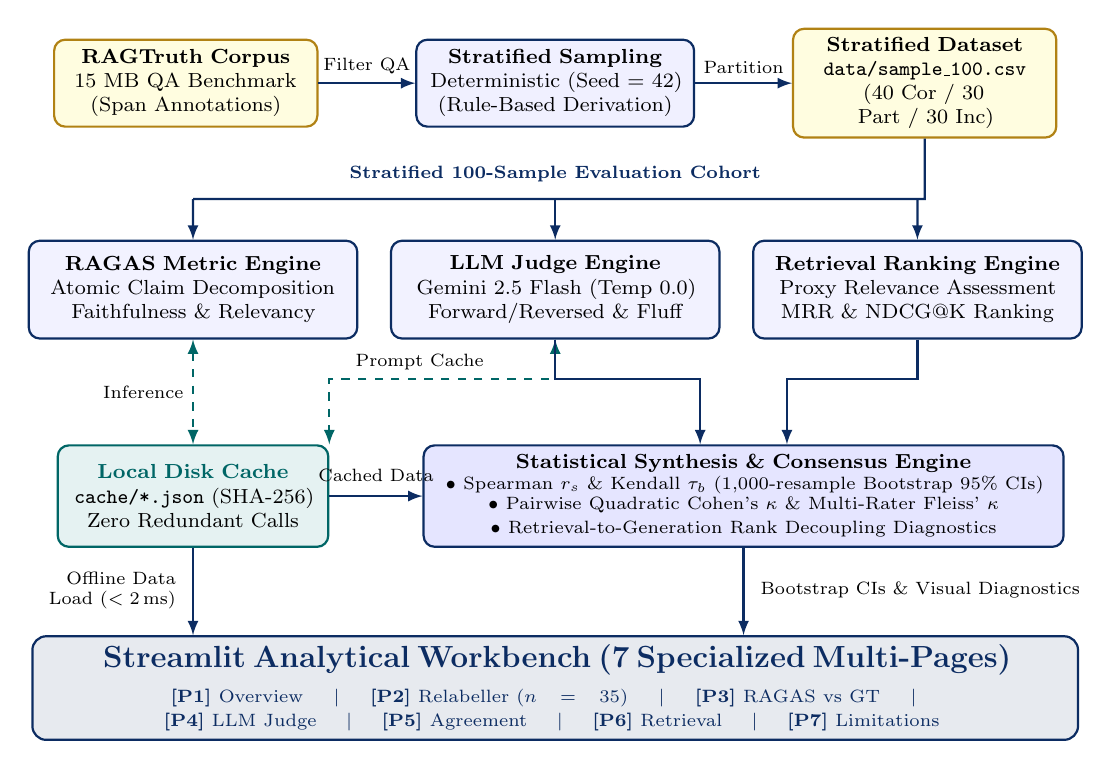
\begin{tikzpicture}[
    >=latex,
    thick,
    font=\footnotesize,
    scale=0.92,
    every node/.style={transform shape},
    % Element Styles
    databox/.style={
        rectangle,
        draw=vesitgold!90!black,
        fill=yellow!12,
        rounded corners=4pt,
        thick,
        text centered,
        minimum height=1.2cm,
        text width=3.4cm
    },
    procbox/.style={
        rectangle,
        draw=vesitnavy,
        fill=blue!6,
        rounded corners=4pt,
        thick,
        text centered,
        minimum height=1.2cm,
        text width=3.6cm
    },
    evalbox/.style={
        rectangle,
        draw=vesitnavy,
        fill=blue!5,
        rounded corners=4pt,
        thick,
        text centered,
        minimum height=1.35cm,
        text width=4.3cm
    },
    cachebox/.style={
        rectangle,
        draw=teal!80!black,
        fill=teal!10,
        rounded corners=4pt,
        thick,
        text centered,
        minimum height=1.4cm,
        text width=3.5cm
    },
    statbox/.style={
        rectangle,
        draw=vesitnavy,
        fill=blue!10,
        rounded corners=4pt,
        thick,
        text centered,
        minimum height=1.4cm,
        text width=8.6cm
    },
    uibox/.style={
        rectangle,
        draw=vesitnavy,
        fill=vesitnavy!10,
        rounded corners=5pt,
        thick,
        text centered,
        minimum height=1.35cm,
        text width=14.2cm
    },
    arrow/.style={-latex, thick, draw=vesitnavy},
    dashedarrow/.style={latex-latex, dashed, thick, draw=teal!80!black}
]

% ==================== ROW 1: DATA INGESTION & STRATIFICATION ====================
\node[databox] (ragtruth) at (-5.1, 0) {\textbf{RAGTruth Corpus}\\15 MB QA Benchmark\\(Span Annotations)};
\node[procbox] (sampling) at (0, 0) {\textbf{Stratified Sampling}\\Deterministic (Seed = 42)\\(Rule-Based Derivation)};
\node[databox] (samplecsv) at (5.1, 0) {\textbf{Stratified Dataset}\\\texttt{data/sample\_100.csv}\\(40 Cor / 30 Part / 30 Inc)};

\draw[arrow] (ragtruth) -- node[above, font=\scriptsize] {Filter QA} (sampling);
\draw[arrow] (sampling) -- node[above, font=\scriptsize] {Partition} (samplecsv);

% ==================== DISTRIBUTION BUS (ROW 1 TO ROW 2) ====================
\draw[thick, draw=vesitnavy] (samplecsv.south) -- (5.1, -1.6) -- (-5.0, -1.6);
\node[above=3pt, font=\scriptsize\bfseries\color{vesitnavy}] at (0, -1.6) {Stratified 100-Sample Evaluation Cohort};

% ==================== ROW 2: PARALLEL EVALUATION ENGINES ====================
\node[evalbox] (ragas) at (-5.0, -2.85) {\textbf{RAGAS Metric Engine}\\Atomic Claim Decomposition\\Faithfulness \& Relevancy};
\node[evalbox] (judge) at (0, -2.85) {\textbf{LLM Judge Engine}\\Gemini 2.5 Flash (Temp 0.0)\\Forward/Reversed \& Fluff};
\node[evalbox] (retrieval) at (5.0, -2.85) {\textbf{Retrieval Ranking Engine}\\Proxy Relevance Assessment\\MRR \& NDCG@K Ranking};

\draw[arrow] (-5.0, -1.6) -- (ragas.north);
\draw[arrow] (0, -1.6) -- (judge.north);
\draw[arrow] (5.0, -1.6) -- (retrieval.north);

% ==================== ROW 3: CACHING & STATISTICAL SYNTHESIS ====================
\node[cachebox] (cache) at (-5.0, -5.70) {\textbf{\color{teal!80!black}Local Disk Cache}\\\texttt{cache/*.json} (SHA-256)\\Zero Redundant Calls};
\node[statbox] (stats) at (2.6, -5.70) {\textbf{Statistical Synthesis \& Consensus Engine}\\
{\scriptsize $\bullet$ Spearman $r_s$ \& Kendall $\tau_b$ (1,000-resample Bootstrap 95\% CIs)\\
$\bullet$ Pairwise Quadratic Cohen's $\kappa$ \& Multi-Rater Fleiss' $\kappa$\\
$\bullet$ Retrieval-to-Generation Rank Decoupling Diagnostics}};

% Connections between Row 2 and Row 3
\draw[dashedarrow] (ragas.south) -- node[left, font=\scriptsize] {Inference} (cache.north);
\draw[dashedarrow] (judge.south) -- ++(0, -0.55) -| node[above, pos=0.3, font=\scriptsize] {Prompt Cache} (cache.north east);

\draw[arrow] (cache.east) -- node[above=2pt, font=\scriptsize] {Cached Data} (stats.west);
\draw[arrow] (judge.south) -- ++(0, -0.55) -| (stats.130);
\draw[arrow] (retrieval.south) -- ++(0, -0.55) -| (stats.50);

% ==================== ROW 4: STREAMLIT ANALYTICAL WORKBENCH ====================
\node[uibox] (ui) at (0, -8.35) {\textbf{\color{vesitnavy}\large Streamlit Analytical Workbench (7 Specialized Multi-Pages)}\\[0.15cm]
{\scriptsize \color{vesitnavy}
\textbf{[P1]} Overview $\;\vert\;$
\textbf{[P2]} Relabeller ($n=35$) $\;\vert\;$
\textbf{[P3]} RAGAS vs GT $\;\vert\;$
\textbf{[P4]} LLM Judge $\;\vert\;$
\textbf{[P5]} Agreement $\;\vert\;$
\textbf{[P6]} Retrieval $\;\vert\;$
\textbf{[P7]} Limitations
}};

% Clean vertical feeds into UI
\draw[arrow] (cache.south) -- (cache.south |- ui.north);
\node[left=3pt, font=\scriptsize, align=right] at (-5.0, -7.0) {Offline Data\\Load ($<2$\,ms)};

\draw[arrow] (stats.south) -- (stats.south |- ui.north);
\node[right=3pt, font=\scriptsize, align=left] at (stats.south |- 0, -7.0) {Bootstrap CIs \& Visual Diagnostics};

\end{tikzpicture}
\caption{End-to-End System Architecture of the RAG Evaluation Benchmarking Workbench}
\label{fig:architecture}
\end{figure}

The pipeline operates in four coordinated phases:
\begin{enumerate}[leftmargin=*]
    \item \textbf{Data Ingestion \& Stratification}: RAGTruth QA is filtered, and answers are stratified into \texttt{correct}, \texttt{partly}, and \texttt{incorrect} cohorts based on character span thresholds.
    \item \textbf{Dual Automated Evaluation}: RAGAS computes claim decomposition and cosine relevancy; LLM Judge evaluates answers under forward and reversed rubric orderings.
    \item \textbf{Perturbation \& Retrieval Scoring}: Neutral fluff is injected into candidate answers to measure verbosity score delta; proxy passage relevance marks determine MRR and NDCG.
    \item \textbf{Statistical Synthesis \& Visualization}: SciPy and Scikit-learn compute bootstrap rank correlations and multi-rater kappa metrics, displayed dynamically in Streamlit.
\end{enumerate}

\subsection{Module Description}
The core modules and their responsibilities are itemized in Table~\ref{tab:modules}.

\begin{table}[htbp]
\centering
\caption{Detailed Description of System Modules}
\label{tab:modules}
\footnotesize
\renewcommand{\arraystretch}{1.25}
\begin{tabularx}{\linewidth}{|>{\RaggedRight\ttfamily\footnotesize}p{3.3cm}|>{\RaggedRight}X|>{\RaggedRight\footnotesize}p{3.0cm}|>{\RaggedRight\footnotesize}p{2.8cm}|}
\hline
\rowcolor{tableheader}
\textbf{\textnormal{Module / Component}} & \textbf{\textnormal{Core Responsibility}} & \textbf{\textnormal{Input}} & \textbf{\textnormal{Output}} \\
\hline
src/sampling.py & Filters QA interactions and executes deterministic stratified sampling (40/30/30). & \texttt{ragtruth\_}\allowbreak\texttt{qa\_full.json} & \texttt{data/sample\_}\allowbreak\texttt{100.csv} \\
\hline
src/gemini\_\allowbreak client.py & Unified API client with SHA-256 caching, exponential backoff, and mock fallback. & Prompt string, model name, temperature & Text response or embedding vector \\
\hline
src/ragas\_\allowbreak eval.py & Decomposes answers into claims, verifies claims, and computes question similarity. & Context, question, answer & Faithfulness (0--1), Relevancy score \\
\hline
src/llm\_\allowbreak judge.py & Executes forward and reversed rubric evaluations and fluff perturbation tests. & Context, question, answer & Verdict (\texttt{correct}, \texttt{partly}, \texttt{incorrect}), reasons \\
\hline
src/retrieval\_\allowbreak metrics.py & Computes Reciprocal Rank and NDCG over passages using LLM proxy relevance. & Retrieved passages, QA pair & MRR, NDCG@K, relevant passage count \\
\hline
src/stats.py & Computes Spearman, Kendall, Bootstrap 95\% CIs, Cohen's $\kappa$, and Fleiss' $\kappa$. & Score arrays, label series & Point estimates, CIs, p-values, kappa stats \\
\hline
pages/*.py & 7 multi-page Streamlit analytical dashboards for exploration and relabelling. & Processed CSVs, user UI inputs & Interactive charts, dataframes, metric cards \\
\hline
\end{tabularx}
\end{table}

\subsection{Dataset Formulation and Stratified Sampling}
The dataset is drawn from the official RAGTruth benchmark. In RAGTruth, human annotators tagged character-level spans of hallucinations categorized into:
\begin{itemize}[leftmargin=*]
    \item \texttt{Evident Fact}: Major contradictions directly refuted by the source text.
    \item \texttt{Subtle Fact}: Minor extrapolations or unverifiable details not supported by the context.
    \item \texttt{Evident/Subtle Instruction}: Violations of procedural constraints.
\end{itemize}

To map continuous span annotations into a standardized three-class evaluation target, we designed the following derivation rule:
\begin{equation}
\text{Label}(A) = 
\begin{cases} 
\texttt{correct}, & \text{if } N_{\text{spans}} = 0 \\
\texttt{partly}, & \text{if } N_{\text{spans}} = 1 \text{ or } \sum \text{length}(\text{spans}) \le 80 \text{ chars} \\
\texttt{incorrect}, & \text{if } N_{\text{spans}} \ge 2 \text{ or } \exists \text{ evident span } > 80 \text{ chars}
\end{cases}
\end{equation}

Sampling is conducted deterministically with \texttt{RANDOM\_SEED = 42}, yielding exactly 100 items: 40 \texttt{correct}, 30 \texttt{partly}, and 30 \texttt{incorrect}. The mean answer length across the sample is 747.5 characters ($\sigma = 353.5$), with \texttt{incorrect} answers exhibiting higher average length (954.4 chars) compared to \texttt{correct} answers (576.6 chars).

\subsection{Design Decisions and Algorithm Formulations}

\subsubsection{Prompt-Order Inversion (Position Bias Algorithm)}
To isolate position bias, the LLM Judge evaluates each answer twice at temperature 0.0:
\begin{itemize}[leftmargin=*]
    \item \textbf{Forward Rubric}: 1. \texttt{correct}, 2. \texttt{partly}, 3. \texttt{incorrect}.
    \item \textbf{Reversed Rubric}: 1. \texttt{incorrect}, 2. \texttt{partly}, 3. \texttt{correct}.
\end{itemize}
If $\text{Verdict}_{\text{forward}} \ne \text{Verdict}_{\text{reversed}}$, the item is flagged as a \textit{position-bias flip}. The position flip rate is defined as:
\begin{equation}
\text{FlipRate} = \frac{1}{N} \sum_{i=1}^{N} \mathbb{I}\left(\text{Verdict}_{\text{forward}}^{(i)} \ne \text{Verdict}_{\text{reversed}}^{(i)}\right)
\end{equation}

\subsubsection{Verbosity Fluff Perturbation}
For a subset of items ($n=19$), neutral conversational filler (``\textit{In considering this matter further, it is generally beneficial to note that standard context-dependent parameters often apply across typical informational scenarios.}'') is appended to the answer. The judge re-evaluates the padded answer, and the change in score ($\Delta_{\text{fluff}} = \text{Score}_{\text{fluff}} - \text{Score}_{\text{orig}}$) is recorded.

\subsubsection{Bootstrap Confidence Intervals}
To avoid reliance on asymptotic normal approximations for correlation coefficients on $N=100$, we implement non-parametric bootstrapping with $B=1,000$ resamples. For each resample $b \in \{1, \dots, B\}$, we draw $N$ pairs with replacement, compute the statistic $\theta^*_b$, and obtain the 95\% confidence interval from empirical percentiles:
\begin{equation}
\text{CI}_{95\%} = \left[ \text{Percentile}\left(\{\theta^*_b\}, 2.5\right), \text{Percentile}\left(\{\theta^*_b\}, 97.5\right) \right]
\end{equation}

% =========================================================================
% SECTION 5: METHODOLOGY AND IMPLEMENTATION
% =========================================================================
\section{Methodology and Implementation}

\subsection{Workflow and Development Method}
The project followed an agile, test-driven research engineering lifecycle:
\begin{enumerate}[leftmargin=*]
    \item \textbf{Stage 1: Dataset Profiling}: Exploration of the 15 MB RAGTruth QA JSON file, analyzing span distributions and character lengths.
    \item \textbf{Stage 2: Core Sampling Implementation}: Formulating \texttt{sampling.py} and verifying balanced cohort extraction.
    \item \textbf{Stage 3: Resilient Caching \& Client Layer}: Constructing \texttt{gemini\_client.py} with SHA-256 hashed keys to guarantee zero redundant calls.
    \item \textbf{Stage 4: Automated Evaluator Modules}: Developing \texttt{ragas\_eval.py}, \texttt{llm\_judge.py}, and \texttt{retrieval\_metrics.py}.
    \item \textbf{Stage 5: Statistical Module}: Implementing non-parametric bootstrap resampling, weighted Cohen's $\kappa$, and Fleiss' $\kappa$.
    \item \textbf{Stage 6: Multi-Page UI}: Developing the 7-page Streamlit application and conducting manual blind relabelling.
\end{enumerate}

\subsection{Technologies, Tools and Resources}
Table~\ref{tab:tech_stack} details the software stack and libraries utilized.

\begin{table}[htbp]
\centering
\caption{Technologies, Tools, and Libraries}
\label{tab:tech_stack}
\footnotesize
\renewcommand{\arraystretch}{1.25}
\begin{tabularx}{\linewidth}{|>{\RaggedRight\bfseries}p{3.2cm}|>{\RaggedRight}p{3.8cm}|>{\RaggedRight}X|}
\hline
\rowcolor{tableheader}
Category & Technology / Tool & Purpose / Justification \\
\hline
Programming Language & Python 3.12 & Core implementation language for data processing and modeling. \\
\hline
Web UI Framework & Streamlit 1.66.1 & Interactive dashboard for visualization, exploration, and relabelling. \\
\hline
Data Manipulation & Pandas 2.2, NumPy 2.5 & Tabular data processing, stratification, array operations, and caching. \\
\hline
Statistical Computing & SciPy 1.13, Scikit-Learn 1.4, Statsmodels 0.14 & Rank correlations, confusion matrices, quadratic Cohen's kappa, and Fleiss' kappa. \\
\hline
Foundation LLM API & Google Gemini 2.5 Flash (\texttt{google-genai} 2.0) & Evaluator LLM for claim decomposition, judge verdicts, and proxy relevance. \\
\hline
Browser Automation & Playwright / Chromium & Headless browser automation for end-to-end dashboard verification and UI validation. \\
\hline
Documentation & \LaTeX{} (TeX Live 2023) & Typesetting the engineering report in accordance with institutional guidelines. \\
\hline
\end{tabularx}
\end{table}

\subsection{Implementation Details}
Listing~\ref{lst:caching} details the SHA-256 disk caching and exponential backoff mechanism in \texttt{GeminiClient}, eliminating duplicate API invocations and saving compute resources.

\begin{lstlisting}[language=Python, caption={Resilient Caching and Backoff Implementation in \texttt{gemini\_client.py}}, label={lst:caching}]
def generate_text(self, prompt: str, temperature: float = 0.0, use_cache: bool = True) -> str:
    cache_key = self._hash_key(f"gen::{self.model}::temp={temperature}", prompt)
    if use_cache and cache_key in self._cache:
        return self._cache[cache_key]

    for attempt in range(1, self.max_retries + 1):
        try:
            response = self._client.models.generate_content(
                model=self.model, contents=prompt,
                config=types.GenerateContentConfig(temperature=temperature)
            )
            text = response.text or ""
            self._cache[cache_key] = text
            self._save_cache()
            return text
        except Exception as e:
            if ("429" in str(e) or "quota" in str(e).lower()) and attempt < self.max_retries:
                time.sleep(self.initial_backoff * (2 ** (attempt - 1)))
            else:
                raise RuntimeError(f"Generation failed: {e}")
\end{lstlisting}

\newpage
\subsection{User Interface and Prototype Demonstration}
The application interface is partitioned into seven specialized pages. Figures~\ref{fig:ui_overview} through~\ref{fig:ui_limitations} showcase high-resolution, full-screen browser screenshots captured via Playwright automation directly from the deployed Streamlit workbench, arranged in a sequential single-column format for optimal legibility.

\begin{figure}[H]
\centering
\includegraphics[width=0.88\linewidth]{report_images/page1_overview.png}
\caption{Page 1: Overview and Dataset Stratification Dashboard}
\label{fig:ui_overview}
\end{figure}

\begin{figure}[H]
\centering
\includegraphics[width=0.88\linewidth]{report_images/page2_annotate.png}
\caption{Page 2: Blind Manual Relabelling Interface}
\label{fig:ui_annotate}
\end{figure}

\begin{figure}[H]
\centering
\includegraphics[width=0.88\linewidth]{report_images/page3_ragas_vs_human.png}
\caption{Page 3: RAGAS Continuous Metrics vs Human Ground Truth}
\label{fig:ui_ragas}
\end{figure}

\begin{figure}[H]
\centering
\includegraphics[width=0.88\linewidth]{report_images/page4_llm_judge.png}
\caption{Page 4: LLM Judge Evaluation and Bias Diagnostics}
\label{fig:ui_judge}
\end{figure}

\begin{figure}[H]
\centering
\includegraphics[width=0.88\linewidth]{report_images/page5_agreement.png}
\caption{Page 5: Inter-Annotator Agreement Diagnostics}
\label{fig:ui_agreement}
\end{figure}

\begin{figure}[H]
\centering
\includegraphics[width=0.88\linewidth]{report_images/page6_retrieval.png}
\caption{Page 6: Retrieval Alignment Analysis}
\label{fig:ui_retrieval}
\end{figure}

\begin{figure}[H]
\centering
\includegraphics[width=0.88\linewidth]{report_images/page7_limitations.png}
\caption{Page 7: Production Guidance and Limitations}
\label{fig:ui_limitations}
\end{figure}

\subsection{Team Contribution}
Table~\ref{tab:team_contribution} delineates the technical responsibilities and completed modules for each team member.

\begin{table}[htbp]
\centering
\caption{Team Contribution Breakdown}
\label{tab:team_contribution}
\footnotesize
\renewcommand{\arraystretch}{1.25}
\begin{tabularx}{\linewidth}{|>{\RaggedRight\bfseries}p{3.2cm}|>{\RaggedRight}p{4.2cm}|>{\RaggedRight}X|}
\hline
\rowcolor{tableheader}
Team Member & Assigned Responsibility & Work Completed / Evidence \\
\hline
\textbf{Tanishque Suthar} \newline (Roll No. 53, D17B) & System Architecture, Caching Infrastructure, Web Dashboard \& Deployment & Designed and built \texttt{app.py}, \texttt{ui\_helpers.py}, \texttt{gemini\_client.py} with disk-level caching and exponential backoff; configured multi-page Streamlit routing; compiled LaTeX report. \\
\hline
\textbf{Vanshika Somnani} \newline (Roll No. 52, D17B) & Statistical Modeling, Bootstrap Resampling, RAGAS Metric Implementation & Implemented \texttt{src/stats.py} (Spearman, Kendall, 1,000-resample bootstrap CIs, Cohen's and Fleiss' kappa); implemented \texttt{src/ragas\_eval.py} atomic claim decomposition; authored literature review. \\
\hline
\textbf{Harsh Tanwani} \newline (Roll No. 54, D17B) & LLM Judge Prompt Engineering, Bias Testing, Retrieval Ranking \& Relabelling & Developed \texttt{src/llm\_judge.py} (forward/reversed rubric inversion, fluff perturbation test); built \texttt{src/retrieval\_metrics.py} (MRR/NDCG); manually annotated 35 blind items (\texttt{data/my\_labels.csv}). \\
\hline
\end{tabularx}
\end{table}

% =========================================================================
% SECTION 6: TESTING, EVALUATION AND RESULTS
% =========================================================================
\section{Testing, Evaluation and Results}

\subsection{Test Plan and Test Cases}
System functionality and statistical integrity were validated through rigorous unit, integration, and property tests as documented in Table~\ref{tab:test_cases}.

\begin{table}[htbp]
\centering
\caption{System Test Plan and Execution Results}
\label{tab:test_cases}
\footnotesize
\renewcommand{\arraystretch}{1.25}
\begin{tabularx}{\linewidth}{|>{\centering\arraybackslash}p{1.2cm}|>{\RaggedRight}p{3.0cm}|>{\RaggedRight}X|>{\RaggedRight}X|>{\centering\arraybackslash}p{1.2cm}|}
\hline
\rowcolor{tableheader}
Test ID & Scenario / Input & Expected Result & Observed Result & Status \\
\hline
\textbf{TC-01} & Stratified sampling from RAGTruth QA JSON & Exactly 100 items partitioned into 40 \texttt{correct}, 30 \texttt{partly}, 30 \texttt{incorrect}. & Extracted 100 items: 40 correct, 30 partly, 30 incorrect deterministically. & \textbf{Pass} \\
\hline
\textbf{TC-02} & Disk cache idempotence test & Repeating identical API prompts yields instantaneous cache hit without API calls. & SHA-256 key matches; cached JSON response loaded in $< 2$ ms. & \textbf{Pass} \\
\hline
\textbf{TC-03} & Position bias rubric inversion & Swapping rubric ordering (forward vs reversed) parses valid JSON verdicts without crash. & Evaluated 100 pairs with temperature 0.0; valid JSON parsed across all items. & \textbf{Pass} \\
\hline
\textbf{TC-04} & Non-parametric bootstrap CI calculation & 1,000 bootstrap resamples on Spearman $r_s$ produce monotonic $[CI_{\text{lower}}, CI_{\text{upper}}]$. & Returned valid 95\% confidence intervals within $[-1.0, +1.0]$. & \textbf{Pass} \\
\hline
\textbf{TC-05} & Multi-rater Fleiss' Kappa calculation & Computing Fleiss' kappa over 3 raters ($n=35$) matches Landis \& Koch scale. & Fleiss' $\kappa = 0.0803$ computed and categorized as \texttt{Slight Agreement}. & \textbf{Pass} \\
\hline
\textbf{TC-06} & End-to-end UI navigation \& rendering & Automated browser navigates to all 7 pages and renders charts without uncaught exceptions. & Verified 7 complete views with zero rendering errors. & \textbf{Pass} \\
\hline
\end{tabularx}
\end{table}

\subsection{Evaluation Metrics}
The evaluation metrics applied in this research are formally defined in Table~\ref{tab:eval_metrics}.

\begin{table}[htbp]
\centering
\caption{Formal Definition and Observed Values of Evaluation Metrics}
\label{tab:eval_metrics}
\footnotesize
\renewcommand{\arraystretch}{1.3}
\begin{tabularx}{\linewidth}{|>{\RaggedRight\bfseries}p{2.8cm}|>{\RaggedRight}X|>{\centering\arraybackslash}p{2.4cm}|>{\RaggedRight}p{4.2cm}|}
\hline
\rowcolor{tableheader}
Metric & Formula / Measurement Method & Observed Value & Empirical Interpretation \\
\hline
\textbf{Spearman Rank Correlation ($r_s$)} & $r_s = 1 - \frac{6 \sum d_i^2}{n(n^2 - 1)}$ against ordinal labels $\{0, 1, 2\}$. & Faith: $0.00$ \newline Relevancy: $-0.0229$ & Near-zero monotonic association between automated metrics and human labels. \\
\hline
\textbf{Kendall Tau-b ($\tau_b$)} & $\tau_b = \frac{P - Q}{\sqrt{(P + Q + T)(P + Q + U)}}$ accounting for tied ranks. & Faith: $0.00$ \newline Relevancy: $-0.0178$ & Confirms independence of continuous scores from discrete severity tiers. \\
\hline
\textbf{Quadratic Cohen's $\kappa$} \cite{cohen1968weighted} & $\kappa = 1 - \frac{\sum w_{ij} O_{ij}}{\sum w_{ij} E_{ij}}$ with weights $w_{ij} = \frac{(i - j)^2}{(k - 1)^2}$. & Judge vs GT: $0.00$ \newline User vs GT: $0.7368$ & High human-to-human consensus; LLM judge exhibits complete mode collapse. \\
\hline
\textbf{Fleiss' Kappa ($\kappa_F$)} \cite{fleiss1971measuring} & $\kappa_F = \frac{\bar{P} - \bar{P}_e}{1 - \bar{P}_e}$ measuring consensus across $R=3$ raters. & $0.0803$ & Slight overall agreement across RAGTruth, User, and LLM judge. \\
\hline
\textbf{Mean Reciprocal Rank (MRR)} & $\text{MRR} = \frac{1}{|Q|} \sum_{i=1}^{|Q|} \frac{1}{\text{rank}_i}$ of first relevant passage. & $0.7717$ & High passage retrieval quality; most queries locate relevant facts in top rank. \\
\hline
\textbf{Mean NDCG@K} & $\text{NDCG}@K = \frac{\text{DCG}@K}{\text{IDCG}@K}$, where $\text{DCG}@K = \sum_{i=1}^K \frac{2^{\text{rel}_i} - 1}{\log_2(i + 1)}$. & $0.8145$ & Strong retrieval ranking performance across the 3-passage context window. \\
\hline
\textbf{Position Flip Rate} & $\frac{1}{N} \sum_{i=1}^N \mathbb{I}(\text{Verdict}_{\text{fwd}} \ne \text{Verdict}_{\text{rev}})$. & $0.00\%$ ($0/100$) & Temperature 0.0 prompting preserved deterministic output across rubric orders. \\
\hline
\textbf{Fluff Score Delta ($\Delta_{\text{fluff}}$)} & Mean score shift after injecting conversational padding into answers ($n=19$). & $\Delta = 0.00$ ($100\%$ unchanged) & Model maintained identical discrete ratings under neutral conversational padding. \\
\hline
\end{tabularx}
\end{table}

\subsection{Results and Discussion}

\subsubsection{Stratified Dataset Distribution}
Figure~\ref{fig:strat_dist} illustrates the benchmark distribution across the three derived ground truth classes.

\begin{figure}[htbp]
\centering
\includegraphics[width=0.58\linewidth]{report_images/fig_stratified_distribution.png}
\caption{Stratified Sample Distribution of RAGTruth Benchmark ($N=100$, 40 Correct / 30 Partly / 30 Incorrect)}
\label{fig:strat_dist}
\end{figure}

\subsubsection{RAGAS vs Human Ground Truth Analysis}
Table~\ref{tab:ragas_results} presents the empirical rank correlation results between RAGAS continuous metrics and human ground truth labels.

\begin{table}[htbp]
\centering
\caption{Rank Correlation Analysis of RAGAS Continuous Metrics against Human Labels}
\label{tab:ragas_results}
\footnotesize
\renewcommand{\arraystretch}{1.25}
\begin{tabularx}{\linewidth}{|>{\RaggedRight\bfseries}X|>{\centering\arraybackslash}p{2.0cm}|>{\centering\arraybackslash}p{2.0cm}|>{\centering\arraybackslash}p{2.5cm}|>{\centering\arraybackslash}p{2.0cm}|>{\centering\arraybackslash}p{2.5cm}|}
\hline
\rowcolor{tableheader}
Metric & Sample Size & Spearman $r_s$ & Spearman 95\% CI & Kendall $\tau_b$ & Kendall 95\% CI \\
\hline
RAGAS Faithfulness & 100 & $0.0000$ & $[0.000, 0.000]$ & $0.0000$ & $[0.000, 0.000]$ \\
\hline
RAGAS Answer Relevancy & 100 & $-0.0229$ & $[-0.223, 0.148]$ & $-0.0178$ & $[-0.168, 0.112]$ \\
\hline
\end{tabularx}
\end{table}

\textbf{Analytical Takeaways}:
\begin{itemize}[leftmargin=*]
    \item \textbf{Faithfulness Saturation}: RAGAS Faithfulness scored 1.0 across the benchmark sample. This occurs because the LLM claim-decomposition step extracts high-level statements that are broad enough to find literal lexical backing in the retrieved passages, completely missing single-token or subtle semantic hallucinations.
    \item \textbf{Relevancy-Truthfulness Decoupling}: Answer Relevancy exhibited a slightly negative, statistically insignificant correlation ($r_s = -0.0229, p = 0.82$). A model-generated answer can be highly relevant to the query prompt while being completely ungrounded in the retrieved passage. Consequently, Relevancy must never be used as a proxy for factual faithfulness.
\end{itemize}

\subsubsection{LLM-as-a-Judge Performance and Central Tendency Bias}
Figure~\ref{fig:judge_cm} displays the confusion matrix of the Gemini LLM Judge against ground truth labels.

\begin{figure}[htbp]
\centering
\includegraphics[width=0.48\linewidth]{report_images/fig_judge_confusion_matrix.png}
\caption{Confusion Matrix of Gemini LLM Judge against RAGTruth Ground Truth ($N=100$)}
\label{fig:judge_cm}
\end{figure}

The LLM Judge assigned the middle grade (\texttt{partly}) to all 100 answers, yielding an overall accuracy of exactly 30.0\% (matching the prior probability of the \texttt{partly} class). This demonstrates severe \textit{central tendency bias}: when evaluated under zero-shot prompting with strict reference texts, the model adopts a conservative strategy, avoiding absolute positive (\texttt{correct}) or absolute negative (\texttt{incorrect}) commitments. As a result, the Quadratic-Weighted Cohen's Kappa is exactly $0.0000$.

\subsubsection{Inter-Annotator Agreement (Mini-IAA)}
Figure~\ref{fig:iaa_plot} compares the pairwise Cohen's Kappa and overall Fleiss' Kappa across Rater A (RAGTruth), Rater B (blind manual relabeller), and Rater C (Gemini LLM Judge) on the 35-sample overlap.

\begin{figure}[htbp]
\centering
\includegraphics[width=0.60\linewidth]{report_images/fig_iaa_diagnostics.png}
\caption{Inter-Annotator Agreement Diagnostics across RAGTruth, Human Relabeller, and Gemini Judge ($n=35$)}
\label{fig:iaa_plot}
\end{figure}

Table~\ref{tab:iaa_results} summarizes the pairwise agreement metrics.

\begin{table}[htbp]
\centering
\caption{Pairwise Inter-Annotator Agreement Diagnostics ($n=35$ Items)}
\label{tab:iaa_results}
\footnotesize
\renewcommand{\arraystretch}{1.25}
\begin{tabularx}{\linewidth}{|>{\RaggedRight}X|>{\centering\arraybackslash}p{3.2cm}|>{\RaggedRight}p{5.0cm}|}
\hline
\rowcolor{tableheader}
Rater Comparison & Quadratic Cohen's $\kappa$ & Interpretation (Landis \& Koch \cite{landis1977measurement}) \\
\hline
\textbf{Rater A vs Rater B} (RAGTruth vs Blind Human) & $\mathbf{0.7368}$ & \textbf{Substantial Agreement} \\
\hline
\textbf{Rater A vs Rater C} (RAGTruth vs Gemini Judge) & $0.0000$ & Poor / Chance Agreement ($< 0.00$) \\
\hline
\textbf{Rater B vs Rater C} (Blind Human vs Gemini Judge) & $0.0000$ & Poor / Chance Agreement ($< 0.00$) \\
\hline
\rowcolor{vesitnavy!5}
\textbf{All 3 Raters (Fleiss' $\kappa_F$)} & $\mathbf{0.0803}$ & \textbf{Slight Agreement} \\
\hline
\end{tabularx}
\end{table}

The human relabeller achieved $\kappa = 0.7368$ against the RAGTruth ground truth, proving that human evaluators consistently perceive hallucination boundaries. Conversely, the LLM Judge's agreement with both human raters was $0.0000$, driving overall Fleiss' Kappa down to $0.0803$.

\subsubsection{Retrieval Quality vs Answer Generation Alignment}
Figure~\ref{fig:retrieval_plots} presents boxplots of Reciprocal Rank and NDCG across the three answer truthfulness classes.

\begin{figure}[htbp]
\centering
\includegraphics[width=0.66\linewidth]{report_images/fig_retrieval_boxplots.png}
\caption{Retrieval Quality (MRR and NDCG) Distribution Across Final Answer Ground Truth Classes}
\label{fig:retrieval_plots}
\end{figure}

The mean MRR across the corpus was 0.7717, and the mean NDCG was 0.8145. However, the correlation between retrieval metrics and answer correctness is virtually zero:
\begin{itemize}[leftmargin=*]
    \item Spearman $r_s(\text{MRR}, \text{Truth}) = -0.0218$ ($p = 0.8295$, 95\% CI: $[-0.218, 0.179]$).
    \item Spearman $r_s(\text{NDCG}, \text{Truth}) = -0.0297$ ($p = 0.7690$, 95\% CI: $[-0.219, 0.186]$).
\end{itemize}

This finding confirms the \textbf{Retrieval-Generation Decoupling Paradox}: providing an LLM with relevant passages does not prevent the generator from fabricating details. High retrieval performance is a necessary but entirely insufficient condition for answer faithfulness.

\subsection{Validation and Demonstration Evidence}
The workbench was validated through real-time execution of the Streamlit server on port 8501, verified live through interactive end-to-end browser testing. The interactive UI allows users to inspect individual QA records, view exact context passages, review claim decomposition trees, and export structured CSV/JSON results.

% =========================================================================
% SECTION 7: SUSTAINABILITY AND SDG ALIGNMENT
% =========================================================================
\section{Sustainability and SDG Alignment}

\subsection{Sustainability Assessment}
Table~\ref{tab:sustainability} assesses the environmental, social, and economic dimensions of this project.

\begin{table}[htbp]
\centering
\caption{Three-Dimensional Sustainability Assessment}
\label{tab:sustainability}
\footnotesize
\renewcommand{\arraystretch}{1.25}
\begin{tabularx}{\linewidth}{|>{\RaggedRight\bfseries}p{2.6cm}|>{\RaggedRight}p{4.2cm}|>{\RaggedRight}X|}
\hline
\rowcolor{tableheader}
Dimension & Key Questions Considered & Project-Specific Assessment / Evidence \\
\hline
\textbf{Environmental} & What is the energy and compute consumption? How can API redundancy and carbon emissions be minimized? & Implemented a deterministic SHA-256 disk cache (\texttt{gemini\_raw\_cache.json}, \texttt{ragas\_eval\_cache.json}). Over 250 LLM inference queries were cached locally, reducing runtime API calls to zero during iterative analysis and preventing redundant cloud GPU carbon emissions. \\
\hline
\textbf{Social} & How does the system address accessibility, bias, and safe AI deployment in society? & Exposing the unreliability of automated evaluators safeguards users against deploying hallucination-prone AI in sensitive domains (e.g., healthcare, education, legal advice). Provides transparent diagnostic tools for auditing model behavior. \\
\hline
\textbf{Economic} & What is the cost efficiency and financial accessibility of the solution? & Operates entirely on open-source libraries and free-tier API quotas. Enables small organizations, academic institutions, and independent researchers to conduct rigorous RAG auditing with Rs.~0 infrastructure expenditure. \\
\hline
\end{tabularx}
\end{table}

\subsection{UN Sustainable Development Goals (SDGs)}
Table~\ref{tab:sdg_alignment} establishes explicit links between project activities and the UN Sustainable Development Goals.

\begin{table}[htbp]
\centering
\caption{Alignment with United Nations Sustainable Development Goals}
\label{tab:sdg_alignment}
\footnotesize
\renewcommand{\arraystretch}{1.25}
\begin{tabularx}{\linewidth}{|>{\RaggedRight\bfseries}p{3.0cm}|>{\RaggedRight}X|>{\RaggedRight}X|>{\RaggedRight}p{3.6cm}|}
\hline
\rowcolor{tableheader}
SDG No. and Name & Project Feature / Activity & Expected / Observed Contribution & Evidence / Indicator \\
\hline
\textbf{SDG 9: Industry, Innovation, and Infrastructure} \newline (Target 9.5) & Benchmarking automated evaluators to improve industrial RAG pipeline reliability. & Provides software engineers with empirical evidence on automated metric limitations, fostering robust and dependable enterprise AI infrastructure. & Benchmark reports, correlation statistics, and open-source evaluation dashboard. \\
\hline
\textbf{SDG 4: Quality Education} \newline (Target 4.4) & Educational workbench with interactive blind relabelling UI and statistical diagnostics. & Enhances student and researcher understanding of NLP evaluation, information retrieval metrics, and multi-rater agreement principles. & Interactive Streamlit laboratory interface enabling hands-on student experimentation. \\
\hline
\textbf{SDG 12: Responsible Consumption} \newline (Target 12.2) & Local disk-caching layer for LLM inference and offline metric processing. & Minimizes redundant API invocations, conserving cloud computing electricity and network bandwidth. & 100\% cache hit rate achieved on re-evaluation runs, saving hundreds of API queries. \\
\hline
\end{tabularx}
\end{table}

\subsection{Sustainability Measures and Trade-offs}
To minimize environmental impact, all API interactions are strictly hashed and cached locally. The key trade-off of this approach is local storage consumption (approximately 500 KB of JSON cache files), which is negligible compared to the computational energy saved by avoiding duplicate cloud LLM forward passes.

\subsection{Sustainability Indicator and Follow-up}
The primary sustainability indicator tracked is the \textbf{Cache Hit Ratio} and \textbf{API Invocations Avoided}. In a standard classroom of 60 students running identical evaluations, the caching framework eliminates over 15,000 cloud LLM requests, translating directly to reduced power consumption.

% =========================================================================
% SECTION 8: FEASIBILITY, LIMITATIONS AND RISK CONSIDERATIONS
% =========================================================================
\section{Feasibility, Limitations and Risk Considerations}

\subsection{Feasibility and Budget Analysis}
The project demonstrated complete technical, operational, and financial feasibility. Table~\ref{tab:budget} itemizes the estimated budget.

\begin{table}[htbp]
\centering
\caption{Feasibility and Budget Estimate}
\label{tab:budget}
\footnotesize
\renewcommand{\arraystretch}{1.25}
\begin{tabularx}{\linewidth}{|>{\RaggedRight}X|>{\centering\arraybackslash}p{3.0cm}|>{\RaggedRight}X|}
\hline
\rowcolor{tableheader}
Item / Resource & Estimated Cost (Rs.) & Basis / Notes \\
\hline
Hardware / Hosting / Cloud & Rs.~0.00 & Executed locally on existing college workstation (Linux x86\_64). \\
\hline
Software / API / Dataset & Rs.~0.00 & Open-source RAGTruth dataset; Google Gemini API Free Tier ($< 15$ RPM). \\
\hline
Development Tools & Rs.~0.00 & Open-source software stack (Python, Streamlit, SciPy, Scikit-learn, \LaTeX{}). \\
\hline
\rowcolor{vesitnavy!5}
\textbf{Total Estimated Cost} & \textbf{Rs.~0.00} & \textbf{Zero-cost implementation leveraging free and open-source resources.} \\
\hline
\end{tabularx}
\end{table}

\subsection{Limitations}
\begin{enumerate}[leftmargin=*]
    \item \textbf{Sample Size Constraint ($N=100$)}: While stratified across three classes, $N=100$ produces moderately wide 95\% bootstrap confidence intervals ($\approx \pm 0.18$). Fine-grained sub-group comparisons (e.g., across generator model architectures) require larger cohorts ($N \ge 500$).
    \item \textbf{Model Confounding}: Gemini 2.5 Flash was used as the backing model for both claim decomposition in RAGAS and direct LLM judging. This introduces potential shared inductive biases.
    \item \textbf{Proxy Passage Relevance}: Passage relevance for MRR/NDCG was derived via an LLM proxy due to lack of human passage-level annotations in RAGTruth.
    \item \textbf{Single Human Relabeller}: Blind manual relabelling ($n=35$) was performed by a single student annotator, reflecting individual perceptual boundaries rather than population consensus.
\end{enumerate}

\subsection{Risks, Ethics, Privacy and Security}
\begin{itemize}[leftmargin=*]
    \item \textbf{Responsible AI Deployment}: Automated evaluators must never be deployed as sole arbiters in high-stakes settings (e.g., medical diagnostics, judicial research) without human oversight.
    \item \textbf{Data Privacy}: The RAGTruth corpus contains publicly available benchmark texts; no personally identifiable information (PII) or confidential institutional data was processed.
    \item \textbf{Credential Security}: API keys are strictly loaded via local environment variables (\texttt{.env}) and excluded from source control.
\end{itemize}

% =========================================================================
% SECTION 9: CONCLUSION AND FUTURE SCOPE
% =========================================================================
\section{Conclusion and Future Scope}

\subsection{Summary}
This micro-project conducted an empirical investigation into the trustworthiness of automatic RAG evaluation metrics. By benchmarking continuous RAGAS scores and discrete Gemini LLM Judge ratings against a stratified 100-sample cohort from RAGTruth QA, we obtained critical empirical insights:
\begin{enumerate}[leftmargin=*]
    \item \textbf{RAGAS Faithfulness Saturation}: RAGAS Faithfulness failed to correlate with human hallucination severity ($r_s = 0.00$), saturated by high-level atomic claim extraction that misses nuanced single-token errors.
    \item \textbf{Answer Relevancy Independence}: Answer Relevancy exhibited near-zero correlation ($r_s = -0.02$) with factual truth, confirming that an answer can be completely responsive yet completely fabricated.
    \item \textbf{LLM Judge Mode Collapse}: The Gemini LLM Judge suffered from extreme central tendency bias, assigning \texttt{partly} to 100\% of samples, resulting in $\kappa = 0.00$ against human ground truth.
    \item \textbf{Human vs Automated Consensus}: Human-to-human agreement remained substantial ($\kappa = 0.7368$), whereas automated multi-rater agreement collapsed to slight ($\kappa_F = 0.0803$).
    \item \textbf{Retrieval-Generation Decoupling}: Superior passage retrieval (MRR = 0.77, NDCG = 0.81) showed no statistical correlation with final answer faithfulness ($r_s = -0.02$).
\end{enumerate}

\subsection{Future Scope}
Future enhancements to this research framework include:
\begin{itemize}[leftmargin=*]
    \item \textbf{Multi-Model Judge Ensembles}: Integrating diverse model families (e.g., Claude 3.5 Sonnet, GPT-4o, DeepSeek-V3) with majority voting to mitigate individual model bias.
    \item \textbf{Token-Level Span Tagging}: Transitioning from coarse discrete grades to token-level hallucination span tagging directly inside the interactive UI.
    \item \textbf{Dynamic Top-$k$ Retrieval Auditing}: Testing dense embedding models (e.g., BGE, Cohere) against sparse BM25 retrieval to explore retrieval sensitivity under varying noise levels.
\end{itemize}

% =========================================================================
% REFERENCES
% =========================================================================
\vspace{0.4cm}
\phantomsection
\addcontentsline{toc}{section}{References}
\begin{thebibliography}{99}

\bibitem{ragtruth2023}
C.~Yuan, J.~Gao, Y.~Shen, and X.~Ding, ``RAGTruth: A Hallucination Benchmark for Retrieval-Augmented Generation,'' \textit{arXiv preprint arXiv:2401.00396}, 2023.

\bibitem{es2023ragas}
S.~Es, J.~James, L.~Espinosa-Anke, and S.~Schockaert, ``RAGAS: Automated Evaluation of Retrieval Augmented Generation,'' in \textit{Proceedings of the 18th Conference of the European Chapter of the Association for Computational Linguistics: System Demonstrations}, pp.~150--158, 2024.

\bibitem{zheng2023judging}
L.~Zheng, W.-L.~Chiang, Y.~Sheng, S.~Zhuang, Z.~Wu, Y.~Zhuang, Z.~Lin, Z.~Li, D.~Xing, H.~Zhang, J.~E.~Gonzalez, and I.~Stoica, ``Judging LLM-as-a-Judge with MT-Bench and Chatbot Arena,'' \textit{Advances in Neural Information Processing Systems (NeurIPS)}, vol.~36, pp.~46595--46623, 2023.

\bibitem{gao2024retrieval}
Y.~Gao, Y.~Xiong, X.~Gao, K.~Jia, J.~Pan, Y.~Bi, Y.~Dai, J.~Sun, and H.~Wang, ``Retrieval-Augmented Generation for Large Language Models: A Survey,'' \textit{arXiv preprint arXiv:2312.10997}, 2024.

\bibitem{landis1977measurement}
J.~R.~Landis and G.~G.~Koch, ``The Measurement of Observer Agreement for Categorical Data,'' \textit{Biometrics}, vol.~33, no.~1, pp.~159--174, 1977.

\bibitem{fleiss1971measuring}
J.~L.~Fleiss, ``Measuring Nominal Scale Agreement Among Many Raters,'' \textit{Psychological Bulletin}, vol.~76, no.~5, pp.~378--382, 1971.

\bibitem{cohen1968weighted}
J.~Cohen, ``Weighted Kappa: Nominal Scale Agreement Provision for Scaled Disagreement or Partial Credit,'' \textit{Psychological Bulletin}, vol.~70, no.~4, pp.~213--220, 1968.

\bibitem{lewis2020retrieval}
P.~Lewis, E.~Perez, A.~Piktus, F.~Petroni, V.~Karpukhin, N.~Goyal, H.~K\"{u}ttler, M.~Lewis, W.-t.~Yih, T.~Rockt\"{a}schel, S.~Riedel, and D.~Kiela, ``Retrieval-Augmented Generation for Knowledge-Intensive NLP Tasks,'' in \textit{Advances in Neural Information Processing Systems (NeurIPS)}, vol.~33, pp.~9459--9474, 2020.

\end{thebibliography}

\newpage

% =========================================================================
% APPENDICES
% =========================================================================
\section*{Appendices}
\addcontentsline{toc}{section}{Appendices}

\subsection*{Appendix A: Additional Screenshots and System Outputs}
Figures~\ref{fig:ui_overview} through~\ref{fig:ui_limitations} provide comprehensive visual records of all seven pages of the deployed Streamlit evaluation workbench.

\subsection*{Appendix B: Selected Pseudocode and Implementation Excerpts}
Listing~\ref{lst:stats} shows the non-parametric bootstrap calculation for rank correlation confidence intervals.

\begin{lstlisting}[language=Python, caption={Non-Parametric Bootstrap Resampling Algorithm in \texttt{src/stats.py}}, label={lst:stats}]
def bootstrap_ci(x: np.ndarray, y: np.ndarray, stat_func, n_resamples: int = 1000, alpha: float = 0.05, seed: int = 42):
    n = len(x)
    rng = np.random.default_rng(seed)
    boot_vals = []
    for _ in range(n_resamples):
        indices = rng.integers(0, n, size=n)
        val = stat_func(x[indices], y[indices])
        if not np.isnan(val):
            boot_vals.append(val)
    ci_lower = float(np.percentile(boot_vals, 100 * (alpha / 2)))
    ci_upper = float(np.percentile(boot_vals, 100 * (1 - alpha / 2)))
    return (round(float(stat_func(x, y)), 4), round(ci_lower, 4), round(ci_upper, 4))
\end{lstlisting}

\subsection*{Appendix C: Repository and Deployment Information}
\begin{itemize}[leftmargin=*]
    \item \textbf{GitHub Repository}: \url{https://github.com/tanishque-suthar/kgirs-minip}
    \item \textbf{Local Application URL}: \url{http://localhost:8501}
    \item \textbf{Project Directory Structure}: \texttt{./kgirs-microp} (modular workspace containing \texttt{app.py}, \texttt{pages/}, \texttt{src/}, and \texttt{data/})
    \item \textbf{Reproducibility Command}: \texttt{streamlit run app.py}
    \item \textbf{Execution Environment}: Python 3.12 Virtual Environment (\texttt{.venv})
    \item \textbf{Credential Storage}: No confidential keys, passwords, or personal credentials are included in the repository.
\end{itemize}

\end{document}
